% for notes environment
\usepackage{xsavebox}
\usepackage{hyperref}
\usepackage{graphicx}
\usepackage{luatexja}
\usepackage[hiragino-pro,deluxe,nfssonly,jis2004]{luatexja-preset}
\usepackage{fontspec}
\usepackage{epigraph}
\usepackage{etoolbox}
\usepackage{tikz}
\usepackage{framed}
\usepackage{mathtools}
\usepackage{listings}
\usepackage{libertine}
\usepackage[libertine]{newtxmath}
\usepackage{bxcoloremoji}
\usepackage{xcolor}
\usepackage{diagbox}
\usepackage{caption}
\usepackage{appendixnumberbeamer}
\usepackage{braket}
\usepackage{multirow}
\usepackage{xpatch}
\usepackage{multicol}
\usepackage{luatexja-ruby}

\usetikzlibrary{fit}

\setmonofont{CMU Typewriter Text}

\definecolor{links}{HTML}{2A1B81}
\hypersetup{colorlinks,linkcolor=,urlcolor=links}

\usetheme{Boadilla}
\usecolortheme{seahorse}
% \usefonttheme{serif}


\xpatchcmd{\itemize}
  {\def\makelabel}
  {\ifnum\@itemdepth=1\relax
     \setlength\itemsep{1.2ex}% separation for first level
   \else
     \ifnum\@itemdepth=2\relax
       \setlength\itemsep{0.8ex}% separation for second level
       \setlength\topsep{1.2ex}
     \else
       \ifnum\@itemdepth=3\relax
         \setlength\itemsep{0.05ex}% separation for third level
         \setlength\topsep{0.8ex}
   \fi\fi\fi\def\makelabel
  }
 {}
 {}

\setbeamercolor{page number in head/foot}{bg=blue!10}
\setbeamertemplate{footline}{%
  \leavevmode%
  \hbox{%
    \begin{beamercolorbox}[wd=.3\paperwidth,ht=2.25ex,dp=1ex,center]{author in head/foot}%
      \usebeamerfont{author in head/foot}\insertshortauthor\hspace*{1ex}(\insertshortinstitute)
    \end{beamercolorbox}%
    \begin{beamercolorbox}[wd=.2\paperwidth,ht=2.25ex,dp=1ex,center]{title in head/foot}%
      \usebeamerfont{title in head/foot}\insertshorttitle
    \end{beamercolorbox}%
    \begin{beamercolorbox}[wd=.4\paperwidth,ht=2.25ex,dp=1ex,center]{date in head/foot}%
      % \insertshortdate{} @ \InsertConference
      \insertshortdate{}
    \end{beamercolorbox}%
    \begin{beamercolorbox}[wd=.1\paperwidth,ht=2.25ex,dp=1ex,center]{page number in head/foot}%
      \insertframenumber{} / \inserttotalframenumber\hspace*{1ex}
    \end{beamercolorbox}}%
  \vskip0pt%
}

\beamertemplatenavigationsymbolsempty

\setbeamertemplate{bibliography item}{\insertbiblabel}
\setbeamersize{description width=1cm}
\setbeamertemplate{items}[circle]
\setbeamertemplate{section in toc}[circle]
\setbeamertemplate{subsection in toc}{%
  \leavevmode\leftskip=2em
  {%
    \usebeamerfont*{itemize item}%
    \usebeamercolor{subsection number projected}%
    \color{bg}%
    \raise1.25pt\hbox{\donotcoloroutermaths$\bullet$}}%
  \hskip1.5ex\inserttocsubsection\par}

% Definitions for the title page
\newcommand*{\GitHub}[1]{%
  \gdef\InsertGitHub{#1}%
}
\newcommand*{\Email}[1]{%
  \gdef\InsertEmail{\href{mailto:#1}{#1}}%
}
\newcommand*{\Conference}[1]{%
  \gdef\InsertConference{#1}%
}
\setbeamerfont{title}{size=\huge, series=\bfseries, family=\mcfamily\rmfamily}
\setbeamercolor{title}{bg=white}
\setbeamerfont{subtitle}{size=\Large, series=\mdseries, family=\gtfamily\sffamily}
\setbeamerfont{email}{size=\scriptsize, family=\ttfamily}
\setbeamercolor{email}{bg=white}
\setbeamerfont{date}{shape=\itshape, family=\rmfamily}
\setbeamerfont{vc}{size=\scriptsize, family=\ttfamily}
\setbeamercolor{vc}{bg=white}

\renewcommand{\figurename}{Fig}

\input{vc.tex}

\setbeamertemplate{title page}
{%
  \vbox{}
  \vfill
  \begingroup
    \centering
    \hrulefill\par%
    \vskip1ex\par%
    \begin{beamercolorbox}[sep=0pt,center,shadow=false,rounded=true]{title}
      \vfill
      \usebeamerfont{title}\inserttitle\par%
      \ifx\insertsubtitle\@empty%
      \else%
        \vskip0.5ex%
        {\usebeamerfont{subtitle}\usebeamercolor[fg]{subtitle}\insertsubtitle\par}%
      \fi%
      \vfill  
    \end{beamercolorbox}%
    \hrulefill\par%
    \vskip2ex%
    \begin{beamercolorbox}[sep=0pt,center,shadow=false,rounded=true]{author}
      \usebeamerfont{author}\insertauthor
    \end{beamercolorbox}
    \begin{beamercolorbox}[sep=0pt,center,shadow=false,rounded=true]{email}
      \usebeamerfont{email}\InsertEmail
    \end{beamercolorbox}
    \vskip0.1ex
    \begin{beamercolorbox}[sep=5pt,center,shadow=false,rounded=true]{institute}
      \usebeamerfont{institute}\insertinstitute
    \end{beamercolorbox}
    \begin{beamercolorbox}[sep=5pt,center,shadow=false,rounded=true]{date}
      % \usebeamerfont{date}\insertdate \normalfont @ \InsertConference
      \usebeamerfont{date}\insertdate
    \end{beamercolorbox}
    \begin{beamercolorbox}[sep=0pt,center,shadow=false,rounded=true]{vc}
      \usebeamerfont{vc}
      \url{https://github.com/\InsertGitHub} (\texttt{\GITAbrHash})
    \end{beamercolorbox}
    % {\centering
    %   \href{https://creativecommons.org/licenses/by-nc/4.0/}{%
    %     \includegraphics[width=0.1\textwidth]{img/by-nc.pdf}%
    %   }%
    % }
    {\usebeamercolor[fg]{titlegraphic}\inserttitlegraphic\par}
  \endgroup
  \vfill
}
\setbeamertemplate{blocks}[rounded][shadow=false]

% ============ ここを消すとNote消える ================
% \mode<handout>{%
%   \usepackage{pgfpages}
%   \setbeameroption{show notes on second screen=right}
%   \setbeamertemplate{note page}{%
%     \vspace{2ex}\insertnote%
%   }
% }
% ============ ここを消すとNote消える ================


\renewcommand{\kanjifamilydefault}{\gtdefault}

\resetcounteronoverlays{lstlisting}
\definecolor{bluegray}{rgb}{0.4, 0.6, 0.8}
\DeclareCaptionFormat{listing}{{\color{bluegray}\lstlistingname}#2#3}
\captionsetup[lstlisting]{format=listing, font={footnotesize}}

\setmonofont[Ligatures=TeX]{CMU Typewriter Text}

\setbeamertemplate{items}[circle]

\newfontfamily\quotefont[Ligatures=TeX]{Linux Libertine O} % selects Libertine as the quote font

\newcommand*\quotesize{60} % if quote size changes, need a way to make shifts relative
% Make commands for the quotes
\newcommand*{\openquote}
   {\tikz[remember picture,overlay,xshift=0em,yshift=-3ex]
   \node (OQ) {\quotefont\fontsize{\quotesize}{\quotesize}\selectfont``};\kern0pt}

\newcommand*{\closequote}[1]
  {\tikz[remember picture,overlay,xshift=1ex,yshift={#1}]
   \node (CQ) {\quotefont\fontsize{\quotesize}{\quotesize}\selectfont''};}

\newcommand*\shadedauthorformat{\emph} % define format for the author argument

% Now a command to allow left, right and centre alignment of the author
\newcommand*\authoralign[1]{%
  \if#1l
    \def\authorfill{}\def\quotefill{\hfill}
  \else
    \if#1r
      \def\authorfill{\hfill}\def\quotefill{}
    \else
      \if#1c
        \gdef\authorfill{\hfill}\def\quotefill{\hfill}
      \else\typeout{Invalid option}
      \fi
    \fi
  \fi}
% wrap everything in its own environment which takes one argument (author) and one optional argument
% specifying the alignment [l, r or c]
%
\newenvironment{shadequote}[2][l]%
{\hspace{0.5ex}
\authoralign{#1}
\ifblank{#2}
   {\def\shadequoteauthor{}\def\yshift{-1ex}\def\quotefill{\hfill}}
   {\def\shadequoteauthor{\par\authorfill\shadedauthorformat{#2}}\def\yshift{3ex}}
\begin{quote}\normalfont\openquote}
{\shadequoteauthor\quotefill\closequote{\yshift}\end{quote}}

\makeatletter
\def\@fnsymbol#1{\ensuremath{\ifcase#1\or *\or \dagger\or \ddagger\or
   \mathsection\or \mathparagraph\or \|\or **\or \dagger\dagger
   \or \ddagger\ddagger \else\@ctrerr\fi}}
\makeatother

\renewcommand{\thefootnote}{\fnsymbol{footnote}}

\newcommand\ballcircle[1]{%
  {%
    \usebeamercolor{enumerate item}%
    \tikzset{beameritem/.style={circle,inner sep=0,minimum size=2ex,text=enumerate item.bg,fill=enumerate item.fg}}%
    \tikz[baseline=(n.base)]\node(n)[beameritem]{\sffamily#1};%
  }%
}
\newcommand\ballref[1]{%
  \ballcircle{\ref{#1}}%
}

\usetikzlibrary{calc}
\usetikzlibrary{shapes.callouts} 

\pgfkeys{%
    /calloutquote/.cd,
    width/.code                   = {\def\calloutquotewidth{#1}},
    position/.code                = {\def\calloutquotepos{#1}}, 
    author/.code                  = {\def\calloutquoteauthor{#1}},
    at/.code                      = {\def\calloutquoteat{#1}},
    sign/.code                    = {\def\calloutquotesign{#1}},
    /calloutquote/.unknown/.code  = {\let\searchname=\pgfkeyscurrentname
                                      \pgfkeysalso{\searchname/.try=#1,                        
                                      /tikz/\searchname/.retry=#1},\pgfkeysalso{\searchname/.try=#1,
                                      /pgf/\searchname/.retry=#1}
                                    }
}

\makeatletter

\newsavebox\temp@simple@callout@author@box
\newcommand\calloutquote[2][]{%
  \pgfkeys{/calloutquote/.cd,
    width    = 5cm,
    position = {(0.5,-0.2)},
    at       = {(0,0)},
    author   = {},
    sign     = {+}
  }%
  \pgfqkeys{/calloutquote}{#1}%
  \sbox{\temp@simple@callout@author@box}{\mbox{%
    \begin{tabular}{l}
      \calloutquoteauthor%
    \end{tabular}
  }}%
  \node[thin, draw=black!50, rectangle callout,callout relative pointer={\calloutquotepos},align=center,text width=\calloutquotewidth,/calloutquote/.cd,
     #1] (tmpcall) at \calloutquoteat {#2};
  \node at ($ (tmpcall.pointer) - (-\calloutquotesign0.5\wd\temp@simple@callout@author@box,0.7\ht\temp@simple@callout@author@box) $) {\calloutquoteauthor};
}

\newsavebox\temp@simple@callout@box
\newcommand{\simplecallout}[4][{}]{%
  \sbox{\temp@simple@callout@box}{\mbox{%
    \begin{tabular}{l}
      #4%
    \end{tabular}
  }}%
  \begin{center}%
    \begin{tikzpicture}%
      \calloutquote[width=1.05\wd\temp@simple@callout@box,position={(#2.5,-0.2)},fill=#3,rounded corners,author={#1},sign=#2]{
        #4%
      }%
    \end{tikzpicture}%
  \end{center}
}

\makeatother
\newfontfamily{\listingfont}[Scale=0.85]{Menlo}
\definecolor{dkgreen}{rgb}{0,0.6,0}
\definecolor{gray}{rgb}{0.5,0.5,0.5}
\definecolor{mauve}{rgb}{0.58,0,0.82}

\makeatletter
\lst@CCPutMacro\lst@ProcessOther {"2D}{\lst@ttfamily{-{}}{-{}}}
\@empty\z@\@empty
\makeatother

\lstdefinestyle{csharp}{
  numbers=left,
  language=[Sharp]C
}

\lstdefinestyle{cil}{
  numbers=left,
  language=CIL
}

\lstdefinestyle{plain}{
  basicstyle=\listingfont\scriptsize,
  language=Plain,
  showstringspaces=false,
  showtabs=false,
  stringstyle=\listingfont\scriptsize\color{mauve},
  tabsize=2
}

\lstdefinestyle{sh}{
  numbers=left,
  language=sh
}

\lstdefinestyle{c}{
  numbers=left,
  language=C
}

\lstdefinestyle{python}{
  numbers=left,
  language=Python
}

\lstdefinestyle{asm-x86}{
  numbers=left
}

\lstdefinestyle{pseudo-code}{
  numbers=left,
  keywords=[6]{for,from,to,endfor,while,endwhile}
}

\lstdefinestyle{bitcoin-script}{
  mathescape=true
}

\lstset{
  basicstyle=\listingfont,
  frame=single,
  xleftmargin=2em,
  xrightmargin=1em,
  breaklines=true
}

\lstdefinestyle{scala}{
  basicstyle=\listingfont\scriptsize,
  breakatwhitespace=false,
  language=scala,
  captionpos=b,
  commentstyle=\listingfont\scriptsize\color{dkgreen},
  extendedchars=true,
  xleftmargin=1em,
  xrightmargin=1em,
  keepspaces=true,
  keywordstyle=\listingfont\scriptsize\color{blue},
  emphstyle=\listingfont\scriptsize\color{cyan},
  rulecolor=\listingfont\scriptsize\color{black},
  showspaces=false,
  showstringspaces=false,
  showtabs=false,
  stringstyle=\listingfont\scriptsize\color{mauve},
  tabsize=2
}

\lstdefinestyle{go}{
  basicstyle=\listingfont\scriptsize,
  breakatwhitespace=false,
  language=go,
  captionpos=b,
  commentstyle=\listingfont\scriptsize\color{dkgreen},
  extendedchars=true,
  xleftmargin=1em,
  xrightmargin=1em,
  keepspaces=true,
  keywordstyle=\listingfont\scriptsize\color{blue},
  emphstyle=\listingfont\scriptsize\color{cyan},
  rulecolor=\listingfont\scriptsize\color{black},
  showspaces=false,
  showstringspaces=false,
  showtabs=false,
  stringstyle=\listingfont\scriptsize\color{mauve},
  tabsize=2
}

\lstdefinestyle{js}{
  basicstyle=\listingfont\scriptsize,
  breakatwhitespace=false,
  language=JavaScript,
  captionpos=b,
  commentstyle=\listingfont\scriptsize\color{dkgreen},
  extendedchars=true,
  xleftmargin=1em,
  xrightmargin=1em,
  keepspaces=true,
  keywordstyle=\listingfont\scriptsize\color{blue},
  emphstyle=\listingfont\scriptsize\color{cyan},
  rulecolor=\listingfont\scriptsize\color{black},
  showspaces=false,
  showstringspaces=false,
  showtabs=false,
  stringstyle=\listingfont\scriptsize\color{mauve},
  tabsize=2
}

\lstdefinestyle{css}{
  basicstyle=\listingfont\scriptsize,
  breakatwhitespace=false,
  language=CSS,
  captionpos=b,
  commentstyle=\listingfont\scriptsize\color{dkgreen},
  extendedchars=true,
  xleftmargin=1em,
  xrightmargin=1em,
  keepspaces=true,
  keywordstyle=\listingfont\scriptsize\color{blue},
  emphstyle=\listingfont\scriptsize\color{cyan},
  rulecolor=\listingfont\scriptsize\color{black},
  showspaces=false,
  showstringspaces=false,
  showtabs=false,
  stringstyle=\listingfont\scriptsize\color{mauve},
  tabsize=2
}

\lstdefinestyle{html}{
  basicstyle=\listingfont\scriptsize,
  breakatwhitespace=false,
  language=HTML5,
  captionpos=b,
  commentstyle=\listingfont\scriptsize\color{dkgreen},
  extendedchars=true,
  xleftmargin=1em,
  xrightmargin=1em,
  keepspaces=true,
  keywordstyle=\listingfont\scriptsize\color{blue},
  emphstyle=\listingfont\scriptsize\color{cyan},
  rulecolor=\listingfont\scriptsize\color{black},
  showspaces=false,
  showstringspaces=false,
  showtabs=false,
  stringstyle=\listingfont\scriptsize\color{mauve},
  tabsize=2
}

\lstdefinelanguage{Plain}{
  morestring=[b]",
  morestring=[b]'
}

\lstdefinelanguage{scala}{
  morekeywords={abstract,case,catch,class,def,%
    do,else,extends,false,final,finally,%
    for,if,implicit,import,match,mixin,%
    new,null,object,override,package,%
    private,protected,requires,return,sealed,%
    super,this,throw,trait,true,try,%
    type,val,var,while,with,yield},
  moreemph={Byte,Short,Int,Long,Float,Double,Char,
    String,Boolean,Unit,Null,Nothing,Any,AnyRef,
    Left,Right,Either},
  otherkeywords={=>,<-,<\%,<:,>:,\#,@},
  sensitive=true,
  morecomment=[l]{//},
  morecomment=[n]{/*}{*/},
  morestring=[b]",
  morestring=[b]',
  morestring=[b]"""
}

\lstdefinelanguage{golang}%
  {morekeywords=[1]{package,import,func,type,struct,return,defer,panic,%
     recover,select,var,const,iota},%
   morekeywords=[2]{string,uint,uint8,uint16,uint32,uint64,int,int8,int16,%
     int32,int64,bool,float32,float64,complex64,complex128,byte,rune,uintptr,%
     error,interface},%
   morekeywords=[3]{map,slice,make,new,nil,len,cap,copy,close,true,false,%
     delete,append,real,imag,complex,chan,},%
   morekeywords=[4]{for,break,continue,range,go,goto,switch,case,fallthrough,if,%
     else,default,},%
   morekeywords=[5]{Println,Printf,Error,Print,},%
   sensitive=true,%
   morecomment=[l]{//},%
   morecomment=[s]{/*}{*/},%
   morestring=[b]',%
   morestring=[b]",%
   morestring=[s]{`}{`},%
}

\lstdefinelanguage{JavaScript}{%
  keywords={typeof, new, true, false, catch, function, return, null, catch, switch, var, if, in, while, do, else, case, break},
  keywordstyle=\color{blue}\bfseries,
  ndkeywords={class, export, boolean, throw, implements, import, this},
  ndkeywordstyle=\color{darkgray}\bfseries,
  identifierstyle=\color{black},
  sensitive=false,
  comment=[l]{//},
  morecomment=[s]{/*}{*/},
  commentstyle=\color{purple}\ttfamily,
  stringstyle=\color{red}\ttfamily,
  morestring=[b]',
  morestring=[b]"
}

\lstdefinelanguage{CSS}{
  keywords={url},
  morekeywords={@import},
  keywordstyle=\color{blue},
  morecomment=[s]{/*}{*/}
}

\lstdefinelanguage{HTML5}{
    sensitive=true,
    keywords={%
    % JavaScript
    typeof, new, true, false, catch, function, return, null, catch, switch, var, if, in, while, do, else, case, break,
    % HTML
    html, title, meta, style, head, body, script, canvas,
    % CSS
    border:, transform:, -moz-transform:, transition-duration:, transition-property:,
    transition-timing-function:
    },
    % http://texblog.org/tag/otherkeywords/
    otherkeywords={<, >, \/},   
    ndkeywords={class, export, boolean, throw, implements, import, this},   
    comment=[l]{//},
    % morecomment=[s][keywordstyle]{<}{>},  
    morecomment=[s]{/*}{*/},
    morecomment=[s]{<!}{>},
    morestring=[b]',
    morestring=[b]",    
    alsoletter={-},
    alsodigit={:}
}
\newenvironment{notes}
  {%
    \begin{xlrbox}{NotesBox}
    \begin{minipage}{.95\textwidth}
    \small\rmfamily\mcfamily
    \begin{itemize}
    \setlength{\itemindent}{0em}
    \setlength{\footnotesep}{5mm}
  }{%
    \end{itemize}
    \end{minipage}
    \end{xlrbox}
    \note{\theNotesBox}}

\def\AtSOne#1\csod{%
	\begin{array}{c|}
		\hline
		#1\\
		\hline
	\end{array}
}%
\def\AtSTwo#1,#2\csod{%
	\begin{array}{c|c|}
		\hline
		#1 & #2\\
		\hline
	\end{array}
}%
\def\AtSThree#1,#2,#3\csod{%
	\begin{array}{c|c|c|}
		\hline
		#1 & #2 & #3\\
		\hline
	\end{array}
}%
\def\AtSFour#1,#2,#3,#4\csod{%
	\begin{array}{c|c|c|c|}
		\hline
		#1 & #2 & #3 & #4\\
		\hline
	\end{array}
}%
\def\AtSFive#1,#2,#3,#4,#5\csod{%
	\begin{array}{c|c|c|c|c|}
		\hline
		#1 & #2 & #3 & #4 & #5\\
		\hline
	\end{array}
}%
\def\AtSSix#1,#2,#3,#4,#5,#6\csod{%
	\begin{array}{c|c|c|c|c|c|}
		\hline
		#1 & #2 & #3 & #4 & #5 & #6\\
		\hline
	\end{array}
}
\newcommand{\SOne}[1]{\AtSOne#1\csod}
\newcommand{\STwo}[1]{\AtSTwo#1\csod}
\newcommand{\SThree}[1]{\AtSThree#1\csod}
\newcommand{\SFour}[1]{\AtSFour#1\csod}
\newcommand{\SFive}[1]{\AtSFive#1\csod}
\newcommand{\SSix}[1]{\AtSSix#1\csod}

\newcommand\ce[1]{%
  \coloremojiucs{#1}
}

\newcommand*{\lstitem}[1]{
  \setbox0\hbox{\lstinline{#1}}
  \item[\usebox0]
}

\presetkeys{todonotes}{inline, noinlinepar}{}

\title[脱炭素社会の実現に向けて]{%
  \ltjruby{脱炭素社会}{カーボンニュートラル}の実現に向けて
}
\subtitle{これまでの歩みとこれから}
\author[吉村 優]{%
  吉村 優(\textsc{Yoshimura} Hikaru)
}
\Email{yyu@mental.poker}
\date[November 17, 2022]{%
  \oldstylenums{November 17, 2022}
}
\Conference{}
\institute[\InsertEmail]{}
\GitHub{y-yu/carbon-neutral-slide}

\begin{document}

\frame{\maketitle}

\section{はじめに}

\begin{frame}
  \frametitle{はじめに}
  
  \pause
  \begin{itemize}
    \item 世界的に2050年までに\textbf{\ltjruby{脱炭素社会}{カーボンニュートラル}}を目指す動きがある
  \end{itemize}

  \begin{shadequote}[r]{}
    \begin{center}
      排出される二酸化炭素と吸収される二酸化炭素の量が等しい状態の社会
    \end{center}
  \end{shadequote}

  \begin{columns}
    \begin{column}{0.4\textwidth}
      \pause
      \begin{itemize}
        \item 1人1人が\textbf{圧倒的当事者意識}で脱炭素化を進めていく必要がある

        \item このトークでは脱炭素に向けてのこれまでの歩みとこれからについて発表する
      \end{itemize}
    \end{column}
    \begin{column}{0.6\textwidth}
      \begin{figure}[h]
        \centering
        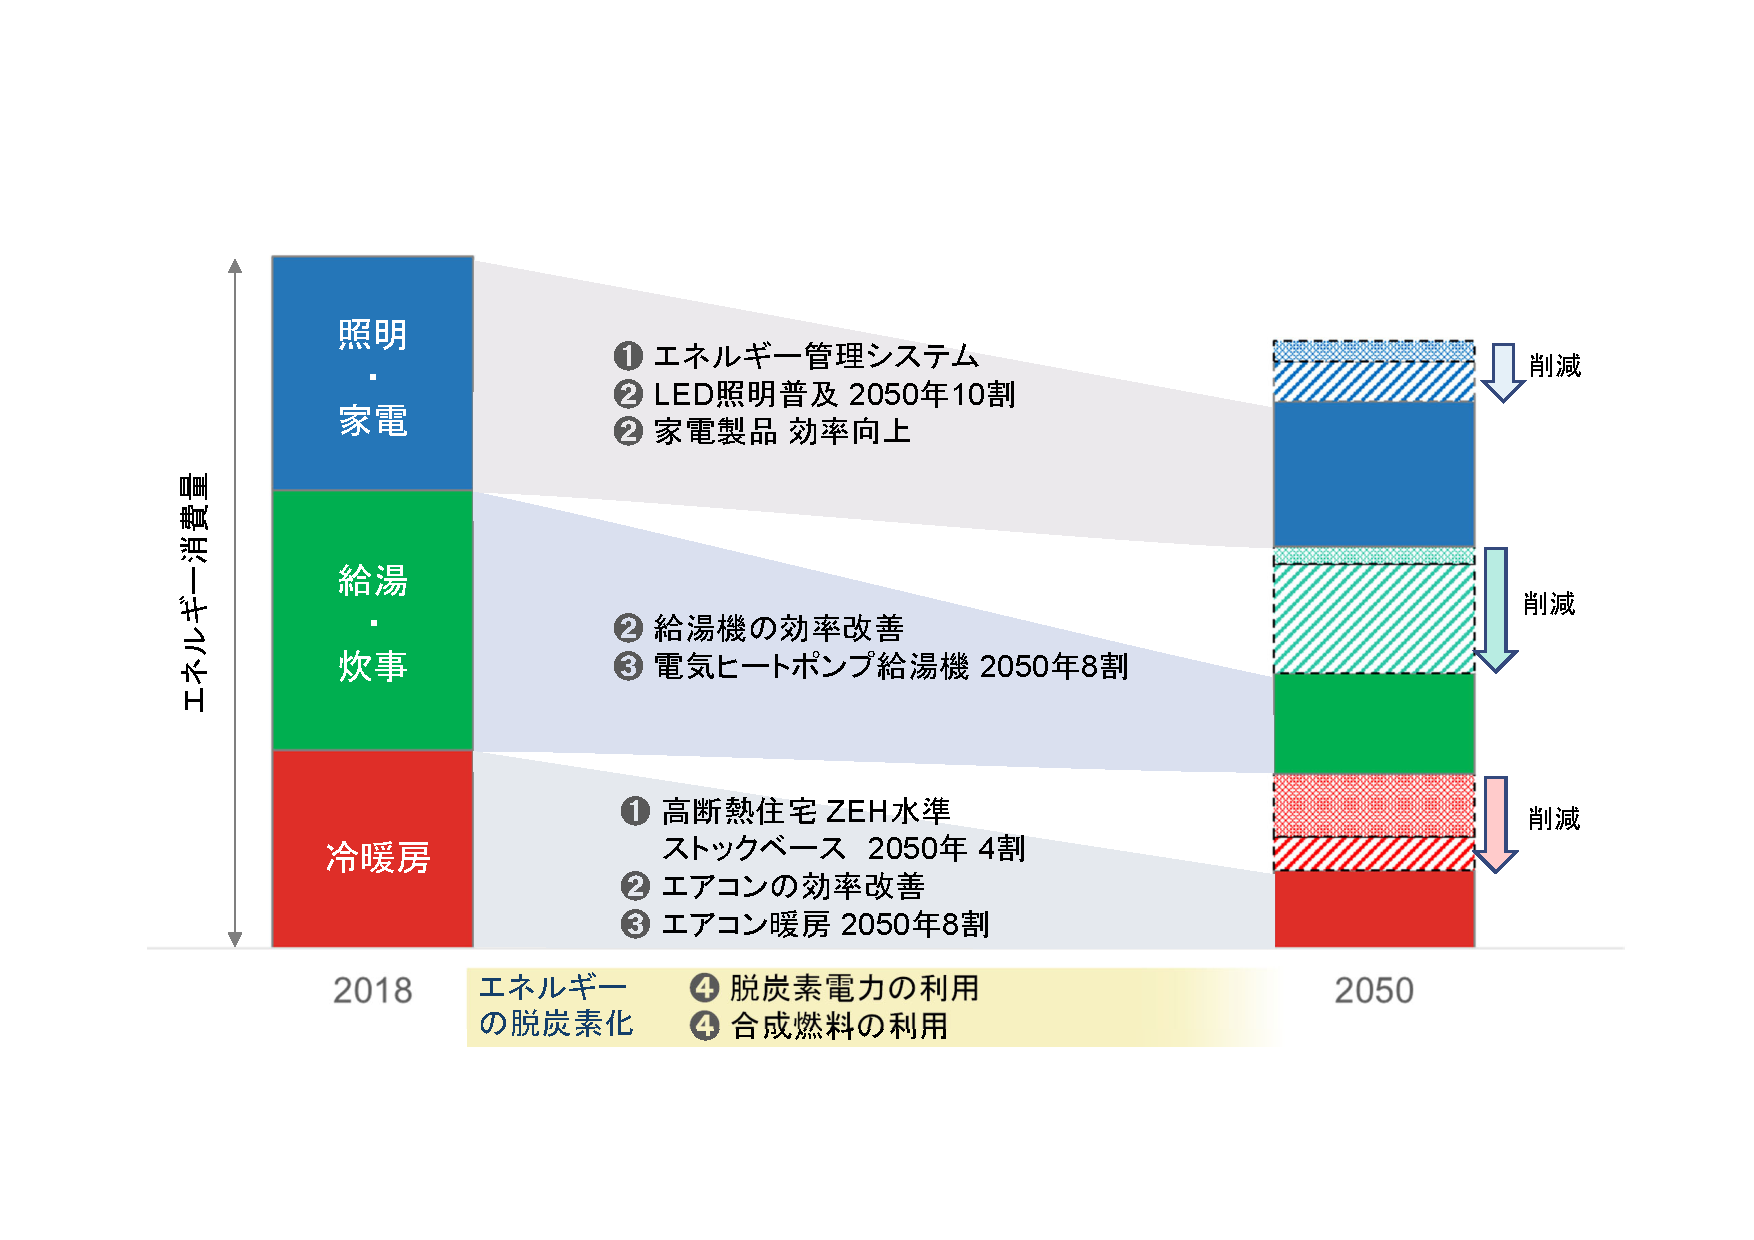
\includegraphics[width=0.75\textwidth]{img/graph.pdf}
        \label{fig:goal_carbon_neutral}
        \caption{脱炭素社会の削減目標\cite{2025_meti}}
      \end{figure}
    \end{column}
  \end{columns}
\end{frame}

\begin{frame}
  \frametitle{脱炭素への取り組みの現状}

  \pause
  \begin{columns}
    \begin{column}{0.6\textwidth}
      \begin{figure}[h]
        \centering
        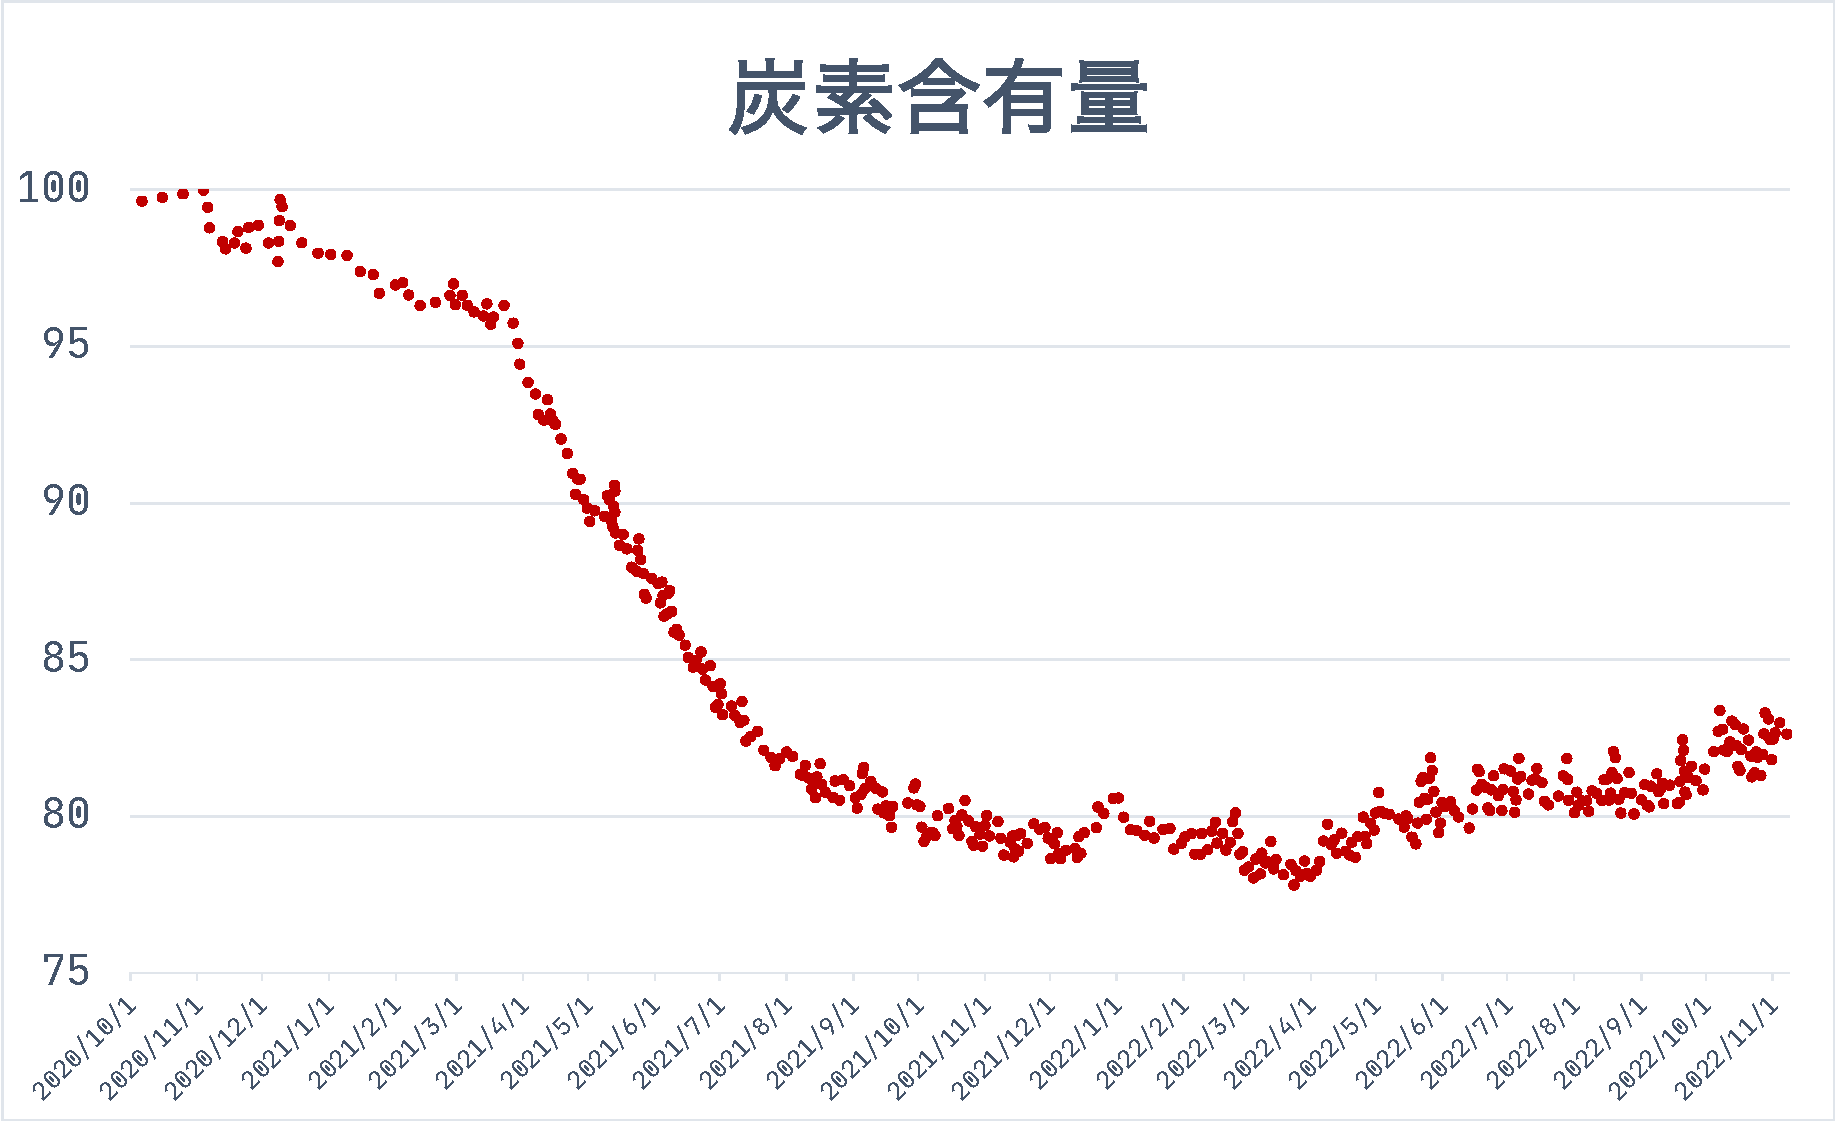
\includegraphics[width=1\textwidth]{img/bodymass.pdf}
        \label{fig:bodymass}
        \caption{炭素含有量の変化}
      \end{figure}
    \end{column}
    \begin{column}{0.4\textwidth}
      \pause
      \begin{itemize}
        \item 2020年10月---2022年11月の\textbf{約2年で約20\%の削減}を実現
      \end{itemize}

      \pause
      \simplecallout[{\Large\ce{:thinking:}}]{+}{cyan!10}{何を行ったのか?}
    \end{column}
  \end{columns}
\end{frame}

\begin{frame}
  \frametitle{目次}

  \begin{columns}
    \begin{column}{0.17\textwidth}
      \begin{minipage}[t][.8\textheight][t]{\textwidth}
        \tableofcontents[currentsection]
      \end{minipage}
    \end{column}
    \pause
    \begin{column}{0.73\textwidth}
      \simplecallout{+}{orange!10}{%
        {\LARGE パーソナルジム\cite{basis}に入会した!}
      }

      \pause
      \uncover<+->{%
        \simplecallout[%
          {
\includegraphics[width=0.2\textwidth]{./img/suppliment_pill_diet.png}}%
        ]{-}{green!10}{%
        {\LARGE ダイエットでやったことを紹介}
      }
    }
    \end{column}
  \end{columns}
\end{frame}


\section{自己紹介}

\begin{frame}
  \frametitle{自己紹介}
  
  \begin{columns}
    \begin{column}{0.3\textwidth}
      \begin{center}
        \begin{figure}
          
\includegraphics[width=0.95\textwidth]{img/bird2x.png}
        \end{figure}
      \end{center}
 
      \begin{table}[h]
        \begin{tabular}{ll}
          Twitter & \href{https://twitter.com/\_yyu\_}{@\_yyu\_} \\
          Qiita &  \href{https://qiita.com/yyu}{yyu} \\
          GitHub &  \href{https://github.com/y-yu}{y-yu} \\
        \end{tabular}
      \end{table}
    \end{column}
    \begin{column}{0.7\textwidth}
      \begin{itemize}
        \item 筑波大学 情報学群 情報科学類卒(2011-15,学士)
        \begin{itemize}
          \item プログラム論理研究室、WORD編集部
        \end{itemize}
        
        \item ドワンゴ ニコニコ動画 アカウントチーム

        \item 未踏ターゲット2018(ゲート式量子コンピュータ)

        \item CTF(\url{https://urandom.team/})
        \begin{itemize}
          \item SECCON CTF 2022で世界57位(国内20位)
        \end{itemize}

        \item プログラミング
        \begin{itemize}
          \item Scala, \LaTeX, Rust, Go, Swift
        \end{itemize}
      \end{itemize}

      \simplecallout[]{-}{red!10}{{\large ダイエットで20kg痩せた!}}
    \end{column}
  \end{columns}
\end{frame}

\begin{frame}
  \frametitle{自己紹介}

  \begin{columns}
    \begin{column}{0.5\textwidth}
      \begin{figure}[h]
        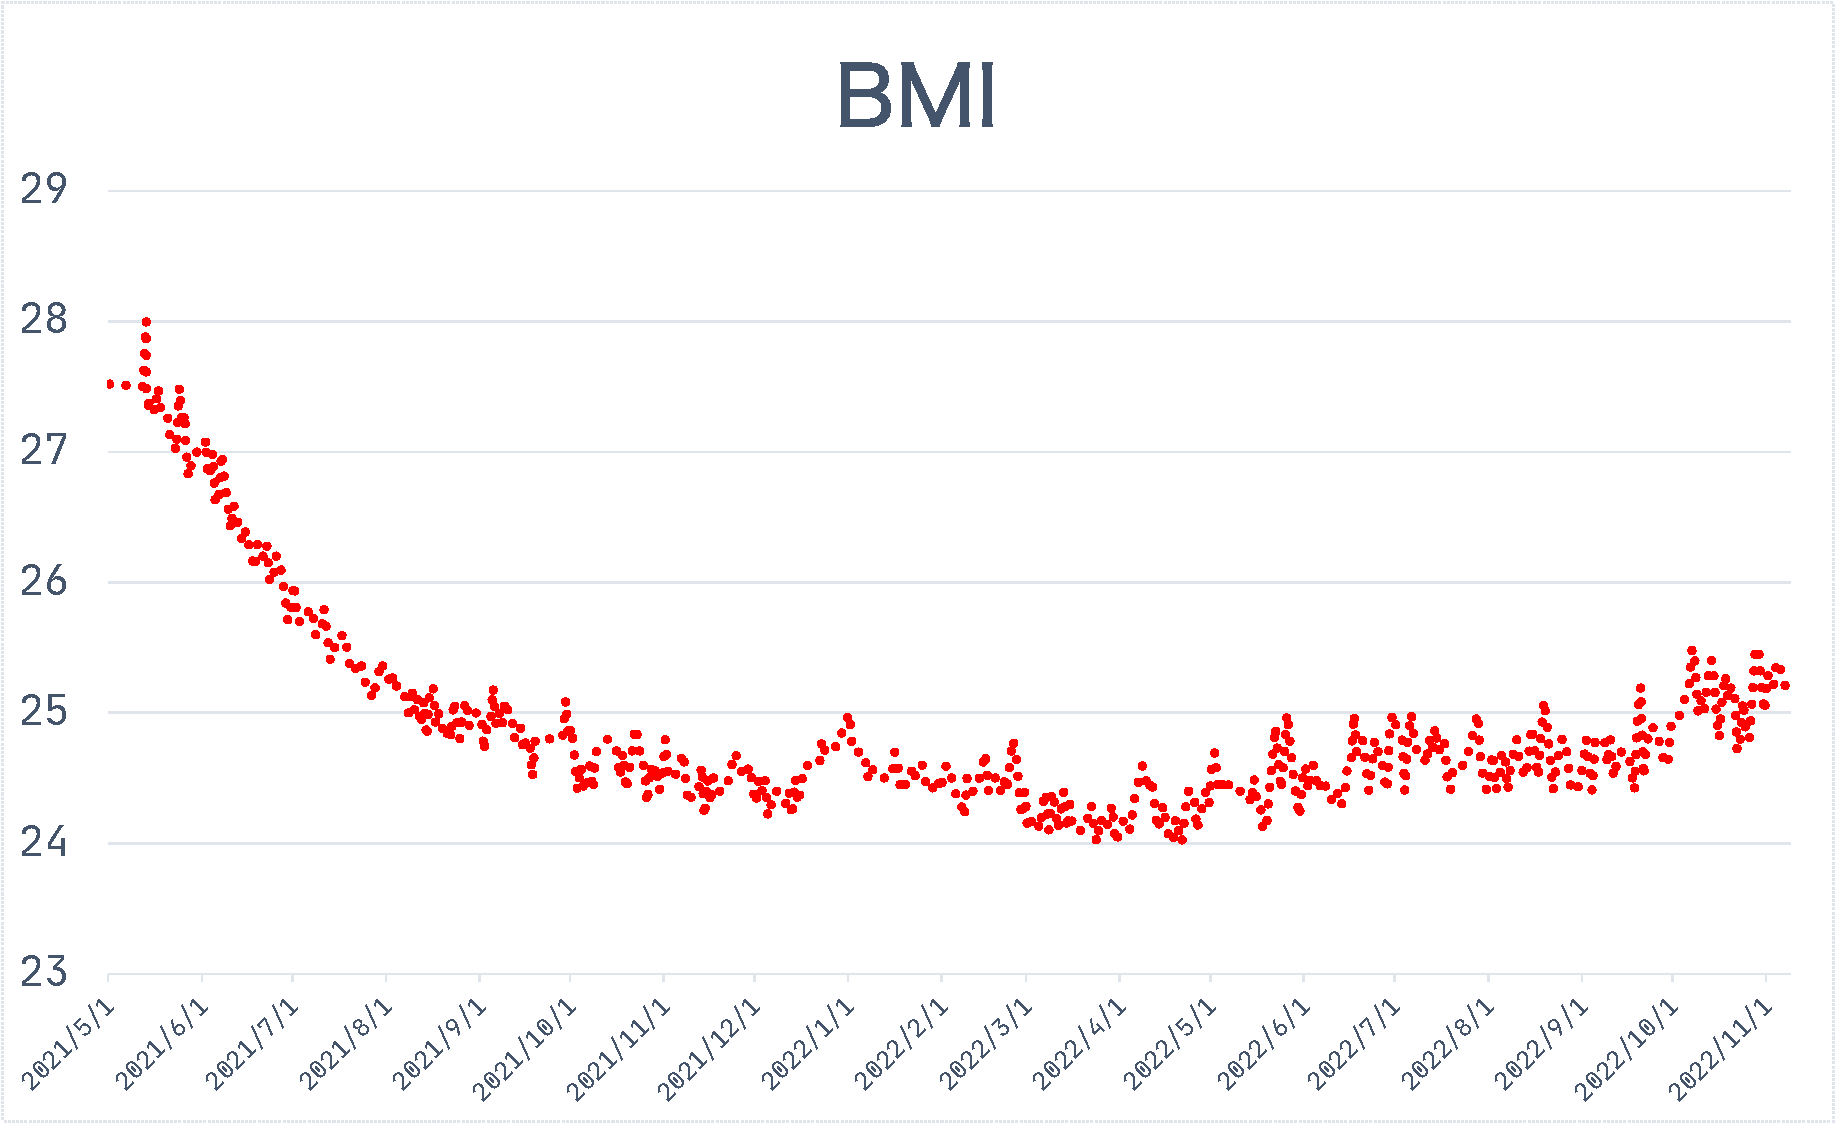
\includegraphics[width=0.95\textwidth]{img/bmi.pdf}
        \label{fig:bmi}
        \caption{BMIの変化}
      \end{figure}

      \simplecallout[]{-}{blue!10}{{\large $28 \rightarrow 25$}}
    \end{column}
    \begin{column}{0.5\textwidth}
      \begin{figure}[h]
        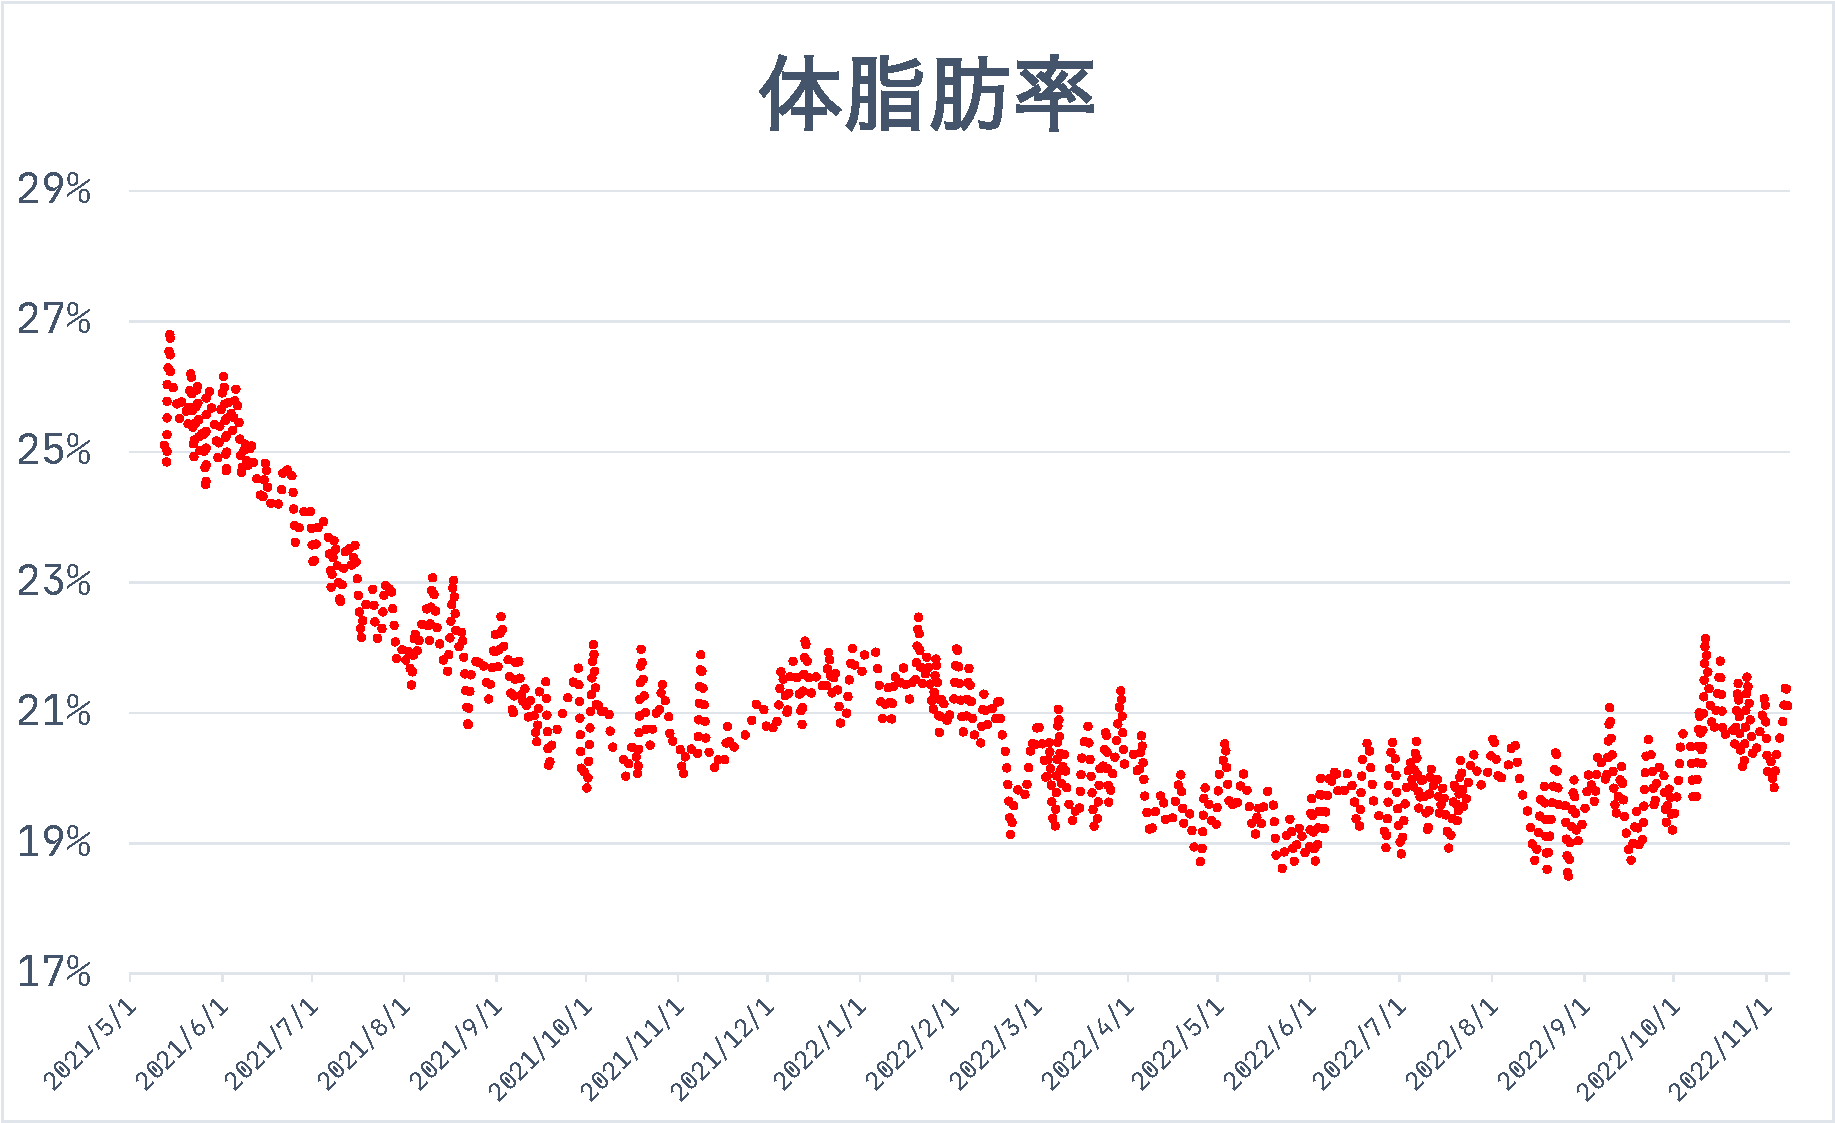
\includegraphics[width=0.95\textwidth]{img/fat_percentage.pdf}
        \label{fig:fat_percentage}
        \caption{体脂肪率の変化}
      \end{figure}

      \simplecallout[]{+}{blue!10}{{\large $27\% \rightarrow 21\%$}}
    \end{column}
  \end{columns}
\end{frame}

\section{ジム}

\begin{frame}
  \frametitle{ジム}

  \begin{itemize}
    \pause
    \item<+-> 90分/週のパーソナルジムに入会した
    \begin{itemize}
      \item コストは4万円/月くらい
      \item 水素水が提供されてなくて近所のジムという基準で選んだ
    \end{itemize}

    \item<+-> ダイエットで体重が減れば基礎代謝も減るため、
    リバウンド対策としてある程度の筋トレがダイエット上も有効
    \begin{itemize}
      \item 筋肉は資産性があり、簡単には減らないため装備しておくと
      食事が増えても大丈夫になる
    \end{itemize}

    \item<+-> (体質によるかもしれないが)筋トレはスポーツとは違って
    最初は雑にやっても割と成果がでてのが嬉しい\ce{:thumbup:}

    \item<+-> どの運動でどの筋肉が利用されるか?といった人体への解像度が向上する
  \end{itemize}
\end{frame}

\section{食事制限}

\begin{frame}
  \frametitle{食事制限}

  \begin{itemize}
    \pause
    \item<+-> ジムのトレーナーにLINEで画像を送る方法で食事を共有していった

    \item<+-> 最初の頃は1500kcal/dayでやっていて相当つらかった
    \begin{itemize}
      \item 現在は1900〜2000kcal/dayくらいかな\ce{:thinking:}
    \end{itemize}

    \item<+-> 個人的には魚\ce{:fish:}は同じカロリーでも体重が増えにくい印象がある

    \item<+-> どの食材がどの程度のカロリーか?ということが分かった
  \end{itemize}
\end{frame}

\section{テコンドー}

\begin{frame}
  \frametitle{テコンドー}

  \pause
  \begin{itemize}
    \item 体重が15kgくらい減って筋肉もついてきた段階で次のような提案があった
    \simplecallout[%
      {
\includegraphics[width=0.1\textwidth]{./img/macho_man.png}}%
    ]{+}{cyan!10}{%
      そろそろ\textit{visual}筋肉か\textit{functional}筋肉か選ぶ時
    }
    \pause
    \begin{description}
      \item[\textit{visual}筋肉] 
      可動域を制約しても外見がよく夏にビーチで使える筋肉

      \item[\textit{functional}筋肉]
      特定のスポーツなどで使える筋肉
    \end{description}

    \begin{itemize}
      \item 筋肉があると外見はよくなるが、大きくて重いので運動でいえば
      少ない筋肉で大量のパワーが出せるのが最もよい
    \end{itemize}

    \item<+-> そういう理由で筋肉の用途としてテコンドー\cite{taekwondo}を初めた
    \begin{itemize}
      \item 90分/週でコストは5000円/月くらい
    \end{itemize}
  \end{itemize}
\end{frame}

\section{これから}

\begin{frame}
  \frametitle{これから}

  \pause
  \begin{itemize}
    \item<+-> これからも下記\ce{:point_down:}の運動は続ける
    \begin{description}
      \item[筋トレ]
      もはや筋トレが目的化しているが今となっても目標を更新できる

      \item[テコンドー]
      人類の歴史において暴力が消えた時代はない

      \item[自転車]
      ダイエットでパワーウェイトレシオが改善された
    \end{description}

    \item<+-> ダイエットや筋トレにお金や時間が必要なのは事実\ce{:innocent:}
    \begin{itemize}
      \item 株や不動産への投資は、受けとるのが将来になるという意味で現在が相対的に薄くなる
      \item 筋肉は比較的少ない時間でキックバックが得られる
      \item 金銭は他人のものを奪って使うことができるが、
    一方で筋肉やそれを得るための知識は奪取することができない
    \end{itemize}

    \item<+-> ジム費用はもはや「食費」と考えるようになった
  \end{itemize}
\end{frame}

\section{まとめ}

\begin{frame}
  \frametitle{まとめ}

  \pause
  \begin{itemize}
    \item<+-> カロリーを制限しつつ運動をすれば痩せる

    \item<+-> リバウンドを警戒するなら、筋トレをやって筋肉をある程度は搭載したほうがいい

    \item<+-> 株や不動産に投資するという考え方もあるが、それと同様にフィジカルに投資するという考え方もある

    \item<+-> ただダイエットは一度はじめたら基本的にはずっとやらないといけないので注意が必要

    \item<+-> 筋トレに興味がある人はSlackの\texttt{\#e\_muscle-ja}にJOIN!
  \end{itemize}
\end{frame}

\section*{参考文献}
\begin{frame}%[allowframebreaks]
  \frametitle{参考文献}
  \nocite{*}
  \bibliographystyle{junsrt_url}
  \bibliography{ref}
\end{frame}

\begin{frame}
  \centering
  {\Huge Thank you for the attention!}
\end{frame}

\end{document}
